% ---------------------------------------
% Freeze action. Определение
%
\ifrender
\tikzstyle{large arrow} = [single arrow,fill=black!20]
\subsection{Freeze action}
\begin{frame}[fragile]{Freeze action}%
\hbsprogresss{0}{0}{1-}{0}{0}{0}{0}{0}{0}%
\hbox to \hsize{\hfil%
\begin{tikzpicture}[auto]%
  \node at (0,0) {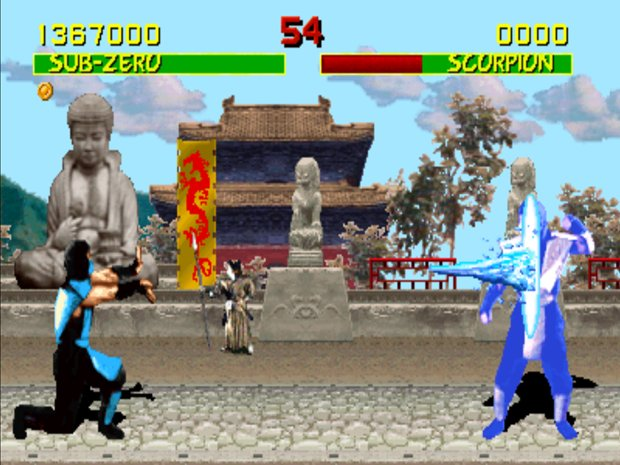
\includegraphics[trim=0 0 0 180,clip,width=0.85\textwidth]{freeze_action.jpg}};
  \node<2-> [large arrow,anchor=mid east] at (3cm, 0.8cm) {\LARGE Freeze action};
  \uncover<3->{\node [large arrow,anchor=mid west,shape border rotate=180] at (5.1cm, -0.5cm) {\LARGE Поле};}
\end{tikzpicture}%
\hfil}%
\\\uncover<3>{Freeze action морозит \lstinline!final! поля в конце конструктора и сразу после их изменения}%
\end{frame}
\fi
